\subsection{Discrete Distributions}

\indent

For any random variable $X$ with a discrete distribution, there is a sample space $\Omega$ with finite or countably infinite number of possible values (outcomes) $x = \{x_1,x_2,...\}$ and associated probabilities $\{p_1,p_2,...\}$.

The point probabilities (aka \textbf{probability mass function}) for each value of $x$ are denoted $f(x)$ and the cumulative distribution function denoted $F(x)$ where:

\begin{align*}
    f(x)=P(X=x),F(x) = P(X<x)
\end{align*}

Properties:

\begin{itemize}
    \item There is a countable number of possible values
    \item $\sum_{i=1}^{\infty}$, where $p_i = f(x_i)=P(X=x_i)$
    \item $0\leq p_i \leq 1$
\end{itemize}

\subsubsection{Binomial Distribution}

\begin{align*}
    S\sim \text{Binomial}(n,p)
\end{align*}

\begin{align*}
    f(s) = 
    \begin{cases}
        (\genfrac{}{}{0pt}{}{n}{s})p^s(1-p)^{n-s},& s=0,1,2,...,n\\
        0,& \text{otherwise}
    \end{cases}
\end{align*}

The $(\genfrac{}{}{0pt}{}{n}{s})$ are known as the binomial coefficients. The parameter $p$ is the probability of success.

\subsection{Continuous Distributions}

\indent

A continuous random variable $X$ is where the outcome can take an infinite (uncountable) number of possible values. These values may be within a fixed or unbounded interval.

The point probabilities for each value of $x$ is $P(X=x)=0$ and the cumulative distribution function:

\begin{align*}
    F(x)=\int_{-\infty}^{x} f(t)dt = P(X\leq x)
\end{align*}

Properties:

\begin{itemize}
    \item There are an uncountable number of possible values.
    \item $f(x)$ is called the probability density function, $f(x)\geq 0$.
    \item $\int_{-\infty}^{\infty}f(x)dx = 1$.
    \item $0\leq f(x)\leq 1$
\end{itemize}

\subsubsection{Normal (Gaussian) Distribution}

\begin{align*}
    X\sim N(\mu,\sigma ^2)
\end{align*}

\begin{align*}
    f(x) = \frac{1}{\sqrt{2\pi}\sigma}e^{-\frac{(x-\mu)^2}{2\sigma^2}}
\end{align*}

\begin{itemize}
    \item $\mu$: the location parameter (mean).
    \item $\sigma$: the scale parameter (sd).
\end{itemize}

\subsection{Density Estimation - Likelihood Approach}

\subsubsection{Density Estimation}

\indent

Suppose random variables $X_1,X_2,...,X_n$ have been observed and assumed to be sampled independently from the distribution with density $f$. \textbf{Goal}: The estimation of the density function $f$.

Applications of density estimation in EDA(exploratory data analysis):

\begin{itemize}
    \item Assess multimodality, skew, tail behaviour, etc.
    \item Decision making, classification, and summarizing Bayesian posteriors.
    \item A useful visualisation tool (a simple summary of a distribution).
\end{itemize}

\subsubsection{Parametric Density Estimation}

\indent

The \textbf{parametric approach} to density estimation assumed parametric model.

\begin{align*}
    X_1,X_2,...,X_n \overset{\text{i.i.d.}}{\sim} f(\theta),\text{ where $\theta$ is a parameter vector}
\end{align*}

\subsubsection{Density Function VS Likelihood Function}

\indent

\textbf{Density Function} $f(X|\theta)$: represents the probability density of observing data $X$ given parameters $\theta$.

\textbf{Likelihood Function} $L(\theta|x)$: is the function used to estimate $\theta$ based on observed data $x$.

\textbf{Maximum likelihood estimator} $\theta_{mle}$: is the value of $\theta$ that maximise the likelihood function

\begin{figure}[h]
    \centering
    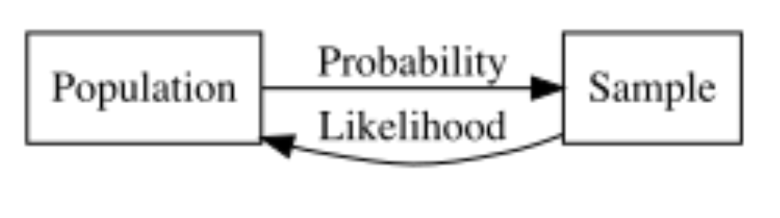
\includegraphics[width=0.5\linewidth]{Figure/Week 3/Likelihood.png}
\end{figure}

\subsubsection{Maximum Likelihood Approach}

\indent

$f(x_1,x_2,...,x_n|\theta)$ is the probability density of observing $x_1,x_2,...,x_n$ given the parameter $\theta$. Assuming independent and identically distributed variables $f(x_1,x_2,...,x_n|\theta)=\prod_{i=1}^{n}f(x_i|\theta)$, maximising the log-likelihood is often easier so it is common to maximise:

\begin{align*}
    L(\theta|x)=\prod_{i=1}^{n}f(x_i|\theta)\xrightarrow{}\mathcal{L}(\theta|x) = \ln{L(\theta|x)} = \sum_{i=1}^{n}\ln{f(x_i|\theta)}
\end{align*}

\subsection{Density Estimation - Non-parametric Approach}

\indent

Danger of misspecification with parametric approach:

\begin{itemize}
    \item If the assumed $f_\theta$ is incorrect
    \item Serious danger of inferential errors
\end{itemize}

Non-parametric approaches to density estimations:

\begin{itemize}
    \item Assume little about the structure of $f$
    \item Use local information to estimate $f$ at a point $x$
\end{itemize}

\subsubsection{Histograms}

\begin{itemize}
    \item One type of nonparametric density estimators.
    \item Piecewise constant density estimators.
    \item Very simple visualization and easy to produce.
    \item \textbf{Sensitive to the number of bins chosen and bin width}.
    \item Preferable to have a smooth estimate and not have columns.
\end{itemize}

\subsubsection{Kernel Density Estimation}

\indent

A kernel is a special type of probability density function (\textbf{PDF}) having the properties:

\begin{align*}
    & K(x)\geq 0 & \text{non-negative}\\
    & K(-x) = K(x)& \text{symmetric} \\
    & \int K(x) dx = 1 & \text{unit measure}
\end{align*}

Kernel density estimation is a non-parametric approach estimating densities. Essentially, \textbf{at every data point, a kernel function is created with the point at its centre}. The PDF is estimated by \textbf{adding all of these kernel functions and dividing by the number of data} to ensure that it satisfies:

\begin{itemize}
    \item Every possible value of the PDF is non-negative
    \item The definite integral of the PDF over its support set equals 1
\end{itemize}

\subsubsection{Kernel Density Estimator (KDE)}

\indent

A simple one weights all points within a window $h$ of $x$ equally:

\begin{align*}
    \hat{f}(x) = \frac{1}{2nh}\sum_{i=1}^{n}1_{\{|X_i-x|<h\}}
\end{align*}

\begin{align*}
\begin{cases}
    1_{A} = 1,& \text{if $A$ is true}\\
    1_{A} = 0,& \text{otherwise}
\end{cases}
\end{align*}

More generally a univariate kernel density estimator has a general weight function (Kernel):

\begin{align*}
    \hat{f}(x) = \frac{1}{nh}\sum_{i=1}^{n}K(\frac{X_i-x}{h})
\end{align*}

\begin{itemize}
    \item $K$ is a kernel function.
    \item $h$ is a bandwidth parameter (possibly fixed or varying).
    \item Consider only $h$ fixed for this course.
\end{itemize}

There are two main components for the KDE: the choice of $K$ and $h$.

\begin{itemize}
    \item The choice of Kernel is less important and generally gives similar results
    \item The choice of bandwidth is \textbf{important} and can \textbf{vary the result greatly}
\end{itemize}

Some standard kernels:

\begin{align*}
    & K(x) = \frac{1}{2}1_{\{|x|\leq 1\}} & \text{Uniform}\\
    & K(x) = \frac{1}{\sqrt{2\pi}}\exp{\{-\frac{x^2}{2}\}} & \text{Gaussian}\\
    & K(x) = \frac{3}{4}(1-x^2)1_{\{|x|\leq 1\}} & \text{Epanechnikov}
\end{align*}

\subsubsection{Choosing the Bandwidth}

\indent

The density estimator(below) is a fixed-bandwidth kernel density estimator since $h$ is constant.

\begin{align*}
    \hat{f}(x) = \frac{1}{nh}\sum_{i=1}^{n}K(\frac{X_i-x}{h})
\end{align*}

\begin{itemize}
    \item \textbf{$h$ too small}: The density estimator will tend to assign probability density too locally near observed data, causing a wiggly estimated density function with many false modes.
    \item \textbf{$h$ too large}: The density estimator will spread probability density contributions too diffusely, causing smooths away important features of $f$.
\end{itemize}

Here is a bias and variance trade-off: a small(large) bandwidth gives high variance(bias).

\subsubsection{Computing Density in R-project}

Base R-project uses command 'density', specify the bandwidth with 'bw' argument:

\begin{lstlisting}[language = R]
density.cbd <- density(x = distance.cbd, bw = 1.25, from = 0, to = 50)
summary(density.cbd)
\end{lstlisting}

\noindent Visualization:

\begin{lstlisting}[language = R]
plot(density.cbd, main = "Distance to CBD")
\end{lstlisting}

\subsection{Mean squared error, Bias, and Variance}

\indent

We can decompose the mean squared error (MSE) into the sum of three quantities: The variance, the squared bias, and the variance of the error:

Assume $Y = f(X)+\epsilon$ and we have an estimator $\hat{f}(X)$ of $f(X)$,

\begin{align*}
    \mathbb{E}(Y-\hat{f}(X))^2 = Var(\hat{f}(X))+[Bias(\hat{f}(X))]^2 + Var(\epsilon)
\end{align*}

where Bias is error introduced by approximating the data using a model.

Variance here denoting how much would $f(x)$ change if we estimate using a different training set.


